\documentclass[a4paper, 12pt]{examen}

\begin{document}

%\modulo{Prog. multim. y de dispositivos moviles}
%\modulo{Planif. y adm. de redes}
%\modulo{Prog. de servicios y procesos}
\modulo{Lenguajes de marcas}

%%%%%%%%%%%%%%%%%%%%%%%%%%%%%%%%%%%%%%%%%%%%%%%%%%%%%%%%%%%%
%%%%%%%%%%%% Recuerda guardar el fichero como ISO-8859-1
%%%%%%%%%%%%%%%%%%%%%%%%%%%%%%%%%%%%%%%%%%%%%%%%%%%%%%%%%%%%

\pregunta{ Elabora un fichero CSS que consiga exactamente
lo que se muestra en la figura \ref{figura1}. Ten en cuenta lo siguiente
{\em y solo lo siguiente}:

\begin{itemize}
\item{Si necesitas posicionar las cajas debes usar exclusivamente float's.}
\item{Observa que el texto de las cajas 1 y 2 queda perfectamente
alineado con los bordes de la caja.}
\item{Los h1 de las cajas 4 y 5 est�n centrados y dichos h1 tambi�n tienen un fondo distinto.}
\item{El tipo de letra de la caja 1 es Helvetica.}
\item{Se ha modificado el espacio que hay entre el borde las cajas y el texto interno, en concreto se
han usado 20px de espacio.}
\item{Recuerda que los m�rgenes y espacios son aproximados, si calculas
por ejemplo un porcentaje de 20 y finalmente fuese 30 esto no perjudica
tu nota. Sin embargo, si hay alg�n espacio, margen, caja mal posicionada
o zona en blanco en la imagen y tu CSS no lo refleja de ninguna forma esto s� restar�}
\end{itemize}

}{3}
\begin{figure}[h]
    \caption{Resultado esperable en el ejercicio 1}
    \label{figura1}
    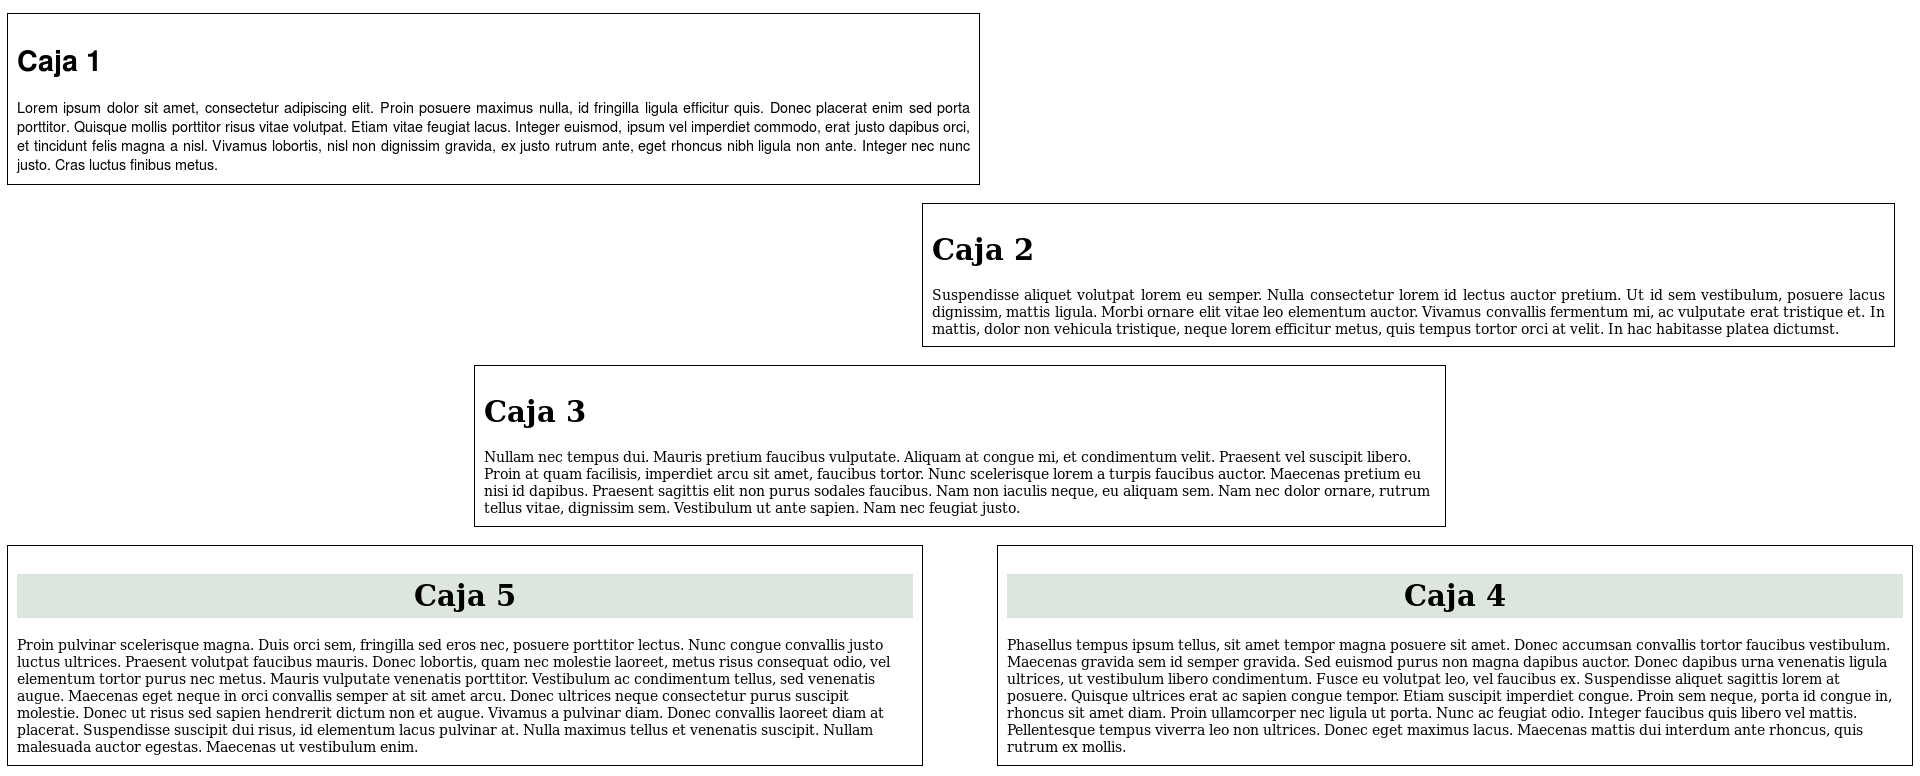
\includegraphics[width=\linewidth]{ej1.png}
\end{figure}
\break

\pregunta{ Elabora un fichero CSS que consiga exactamente
lo que se muestra en la figura \ref{figura2}.
Ten en cuenta lo siguiente:

\begin{itemize}
\item{Se ha usado una rejilla para colocar los elementos. Puedes ver el boceto en la figura \ref{rejilla1}}
\item{Todas las cajas tienen un margen extra de 10px}
\item{Observa que algunos h1 est�n tachados.}

}
\end{itemize}

}{  2.5 }
\begin{figure}[h]
    \caption{Resultado esperable en el ejercicio 2}
    \label{figura2}
    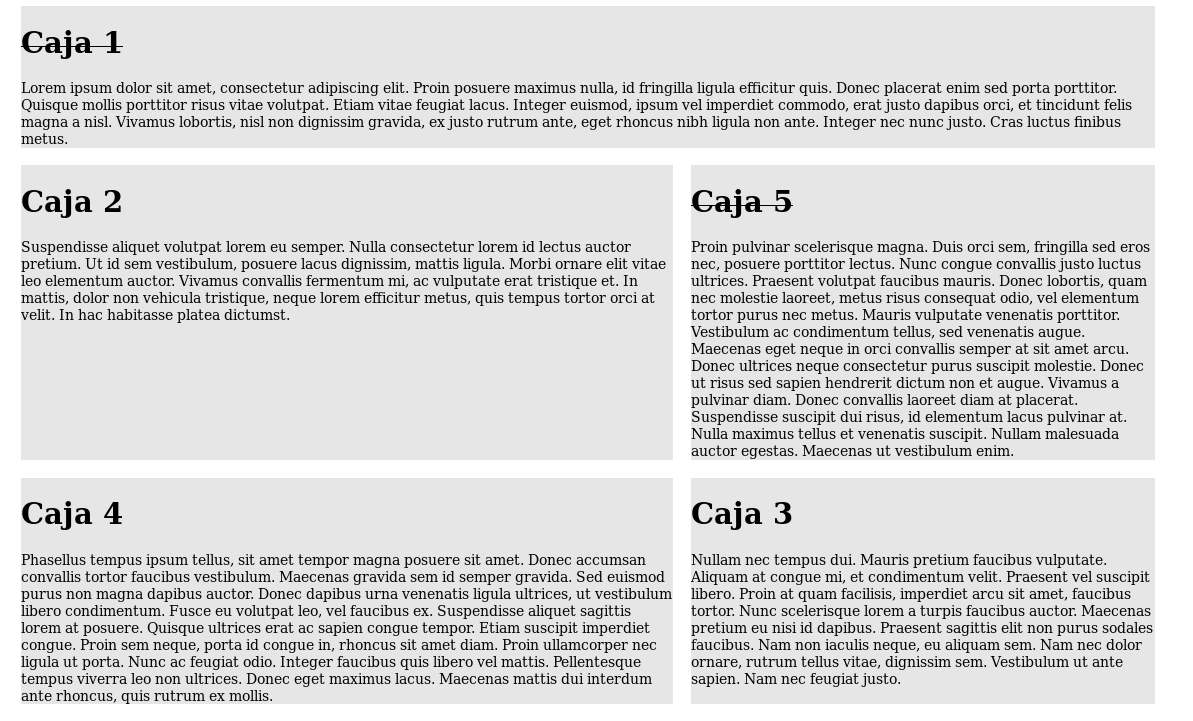
\includegraphics[width=\linewidth]{ej2.png}
\end{figure}

\begin{figure}[h]
    \caption{Rejilla usada para colocar los elementos}
    \label{rejilla1}
    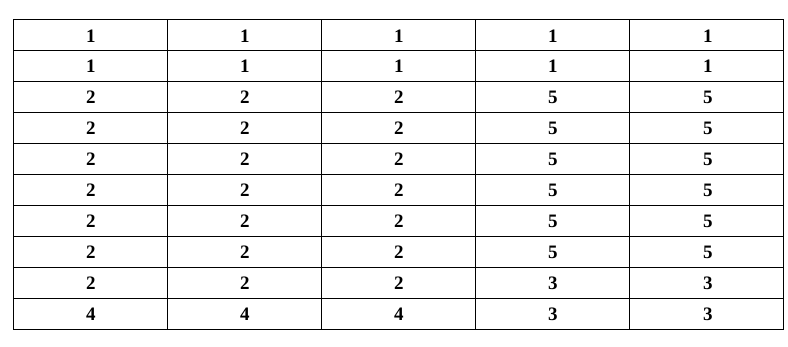
\includegraphics[width=\linewidth]{rejilla.png}
\end{figure}

\break

\pregunta{ Elabora un fichero CSS que consiga lo siguiente para el HTML mostrado.
\begin{itemize}
\item{Puedes a�adir otros elementos HTML o atributos pero {\bf no puedes cambiar el orden}.}
\item{Se han definido dos estilos: uno para pantallas grandes (de 800px en adelante) y otro para peque�as (de menos de 800px)}
\item{En pantallas peque�as:}
    \begin{itemize}
    \item{Se ha modificado el color de los encabezados y se ha usado un tono gris.}
    \item{Se ha cambiado la distancia entre cada caja con respecto a su parte de arriba en 15px.}
    \item{La caja 3 no se muestra. Las cajas 2 y 4 tienen un aspecto distinto al de las cajas 1 y 5.}
    \end{itemize}
\item {En el caso de pantallas grandes:}

\begin{itemize}
    \item{El tipo de letra usado es Arial.}
    \item{{\bf Usando float} las cajas se alinean una al lado de la otra en el orden: 2, 1, 3, 5, 4.}
\end{itemize}
\end{itemize}

}{  4.5 }
\break
\begin{figure}[h]
    \caption{Resultado esperable en el ejercicio 3 (caso 1)}
    \label{figura31}
    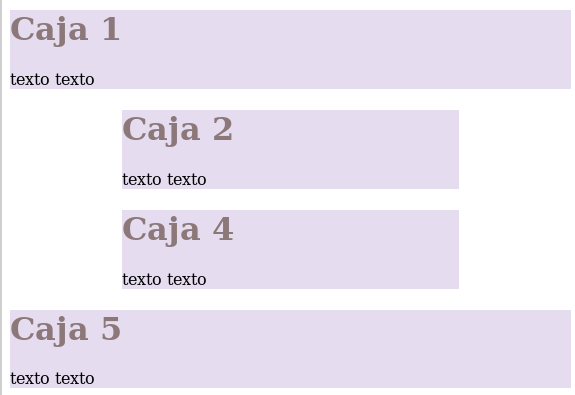
\includegraphics[width=0.8\linewidth]{ej31.png}
\end{figure}

\begin{figure}[h]
    \caption{Resultado esperable en el ejercicio 3 (caso 2)}
    \label{figura32}
    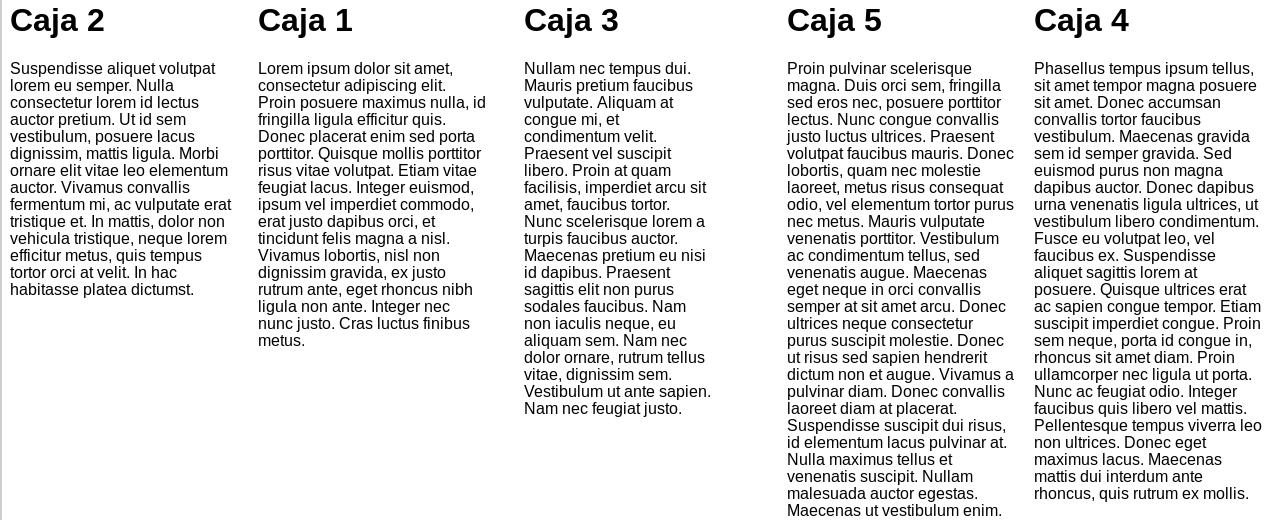
\includegraphics[width=\linewidth]{ej32.png}
\end{figure}


\break
\begin{verbatim}
<div id="caja1"> <!--Ejercicio 1-->
    <h1>Caja 1</h1>
    Texto ...
</div><!--Fin de la caja 1-->
<div id="caja2">
    <h1>Caja 2</h1>
    Texto ...
</div><!--Fin de la caja 2-->
<div id="caja3">
    <h1>Caja 3</h1>
    Texto ...
</div><!--Fin de la caja 3-->
<div id="caja4">
    <h1>Caja 4</h1>
    Texto ...
</div><!--Fin de la caja 4-->
<div id="caja5">
    <h1>Caja 5</h1>
    Texto ...
</div><!--Fin de la caja 5-->
\end{verbatim}

\begin{verbatim}
<div id="caja1"> <!--Ejercicio 2-->
    <h1>Caja 1</h1>
    Texto ...
</div><!--Fin de la caja 1-->
<div id="caja2">
    <h1>Caja 2</h1>
    Texto ...
</div><!--Fin de la caja 2-->
<div id="caja3">
    <h1>Caja 3</h1>
    Texto ...
</div><!--Fin de la caja 3-->
<div id="caja4">
    <h1>Caja 4</h1>
    Texto ...
</div><!--Fin de la caja 4-->
<div id="caja5">
    <h1>Caja 5</h1>
    Texto ...
</div><!--Fin de la caja 5-->
\end{verbatim}

\begin{verbatim}
<div id="caja1"> <!--Ejercicio 3-->
    <h1>Caja 1</h1>
    Texto ...
</div><!--Fin de la caja 1-->
<div id="caja2">
    <h1>Caja 2</h1>
    Texto ...
</div><!--Fin de la caja 2-->
<div id="caja3">
    <h1>Caja 3</h1>
    Texto ...
</div><!--Fin de la caja 3-->
<div id="caja4">
    <h1>Caja 4</h1>
    Texto ...
</div><!--Fin de la caja 4-->
<div id="caja5">
    <h1>Caja 5</h1>
    Texto ...
</div><!--Fin de la caja 5-->
\end{verbatim}
\end{document}
